\begin{frame}
\frametitle{Aufgabe 4}
\framesubtitle{}
    \begin{itemize}
        \item Durch kompliziertere Schaltungen können schärfere
        Frequenztrennungen erreicht werden
        \item Beim Tiefpass wurde fälschlicherweise eine Spule mit $L=100mH$
        verwendet
    \end{itemize}
\end{frame}
\begin{frame}
\frametitle{Aufgabe 4}
\framesubtitle{Tiefpass 2. Ordnung}
\begin{figure}[H]
\begin{center}
        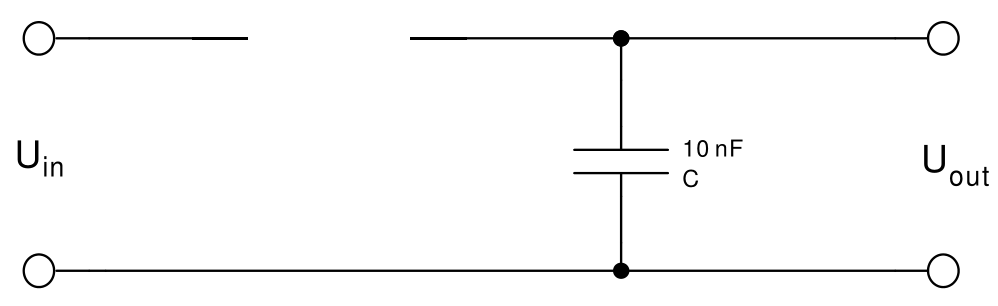
\includegraphics[scale=0.2]{./img/4a_tiefpass_1.png}
\end{center}
\end{figure}
\end{frame}
\begin{frame}
\frametitle{Aufgabe 4}
\framesubtitle{Tiefpass 2.Ordnung}
\begin{figure}[H]
\begin{center}
        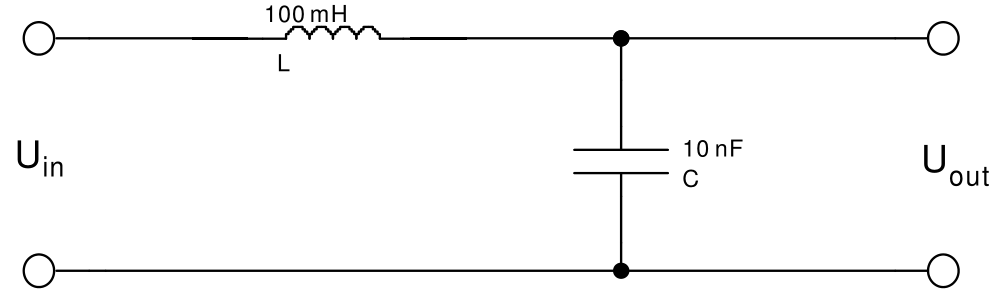
\includegraphics[scale=0.2]{./img/4a_tiefpass_2.png}
\end{center}
\end{figure}
\begin{itemize}
    \item Einbau von Spule
    \item Erwarteter Verlauf
\end{itemize}
\begin{equation*}
    \frac{U_{out}}{U_{in}} = \frac{1}{1-\omega^2 L C}
\end{equation*}
\end{frame}
\begin{frame}
\frametitle{Aufgabe 4}
\framesubtitle{Tiefpass Bode-Diagram}
    \begin{figure}[H]
    \begin{center}
            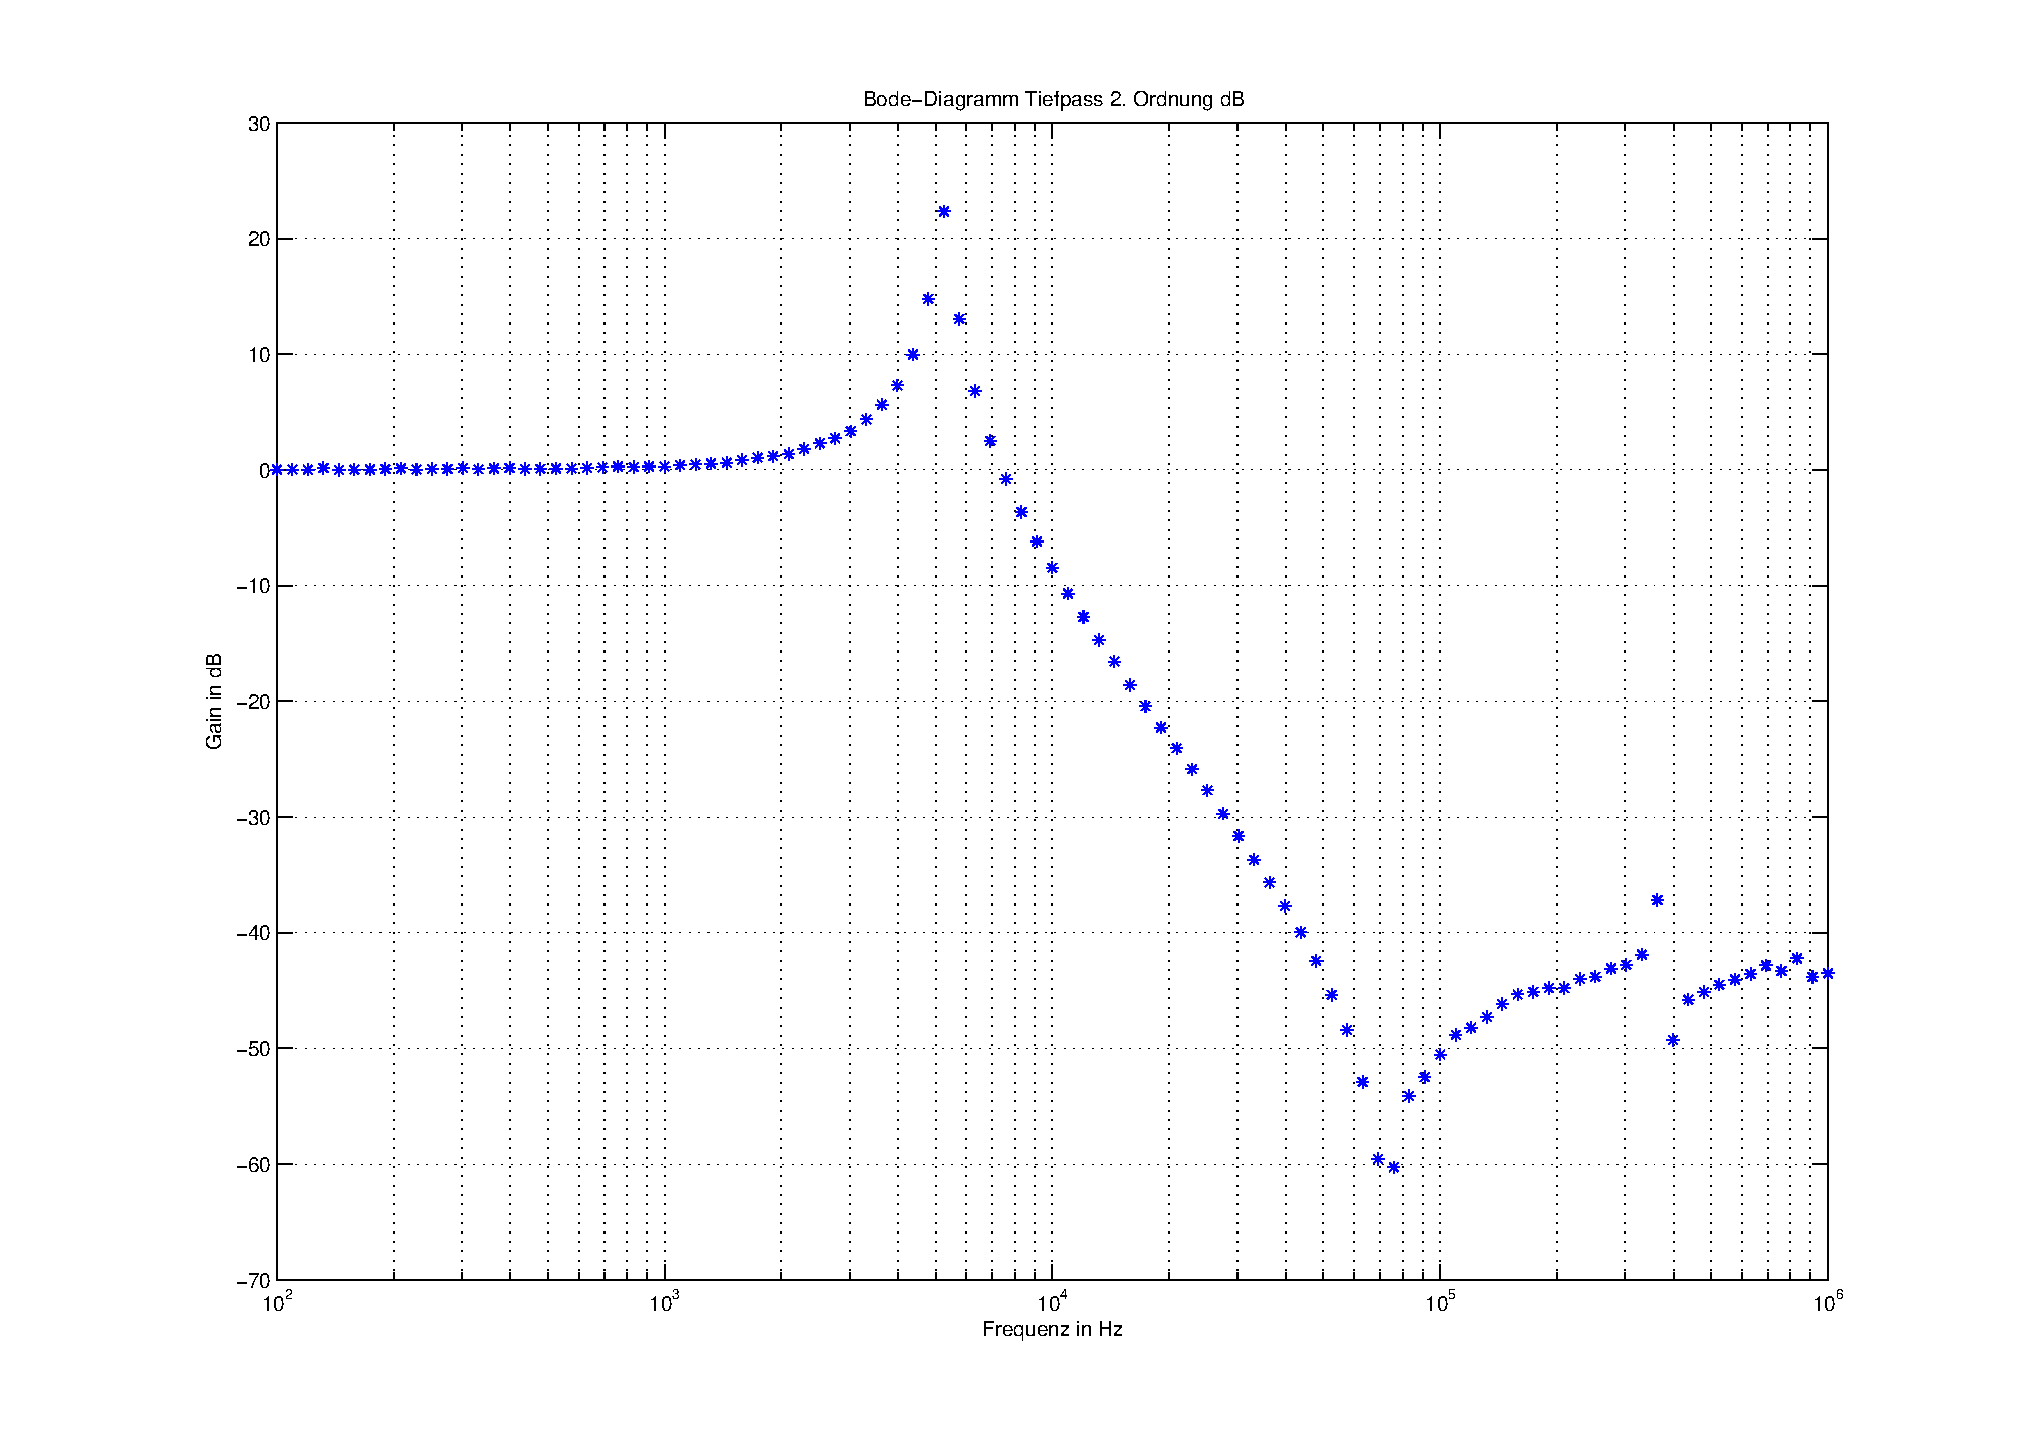
\includegraphics[scale=0.50]{./img/4a_bode_tief_dB.eps}
    \end{center}
    \end{figure}  
\begin{itemize}
    \item Unerwünschte Asymptote bei $\omega = \sqrt{\frac{1}{LC}}$
    \item Schwinkreis ohne Dämpfung
\end{itemize}
\end{frame}
\begin{frame}
    \frametitle{Aufgabe 4}
    \framesubtitle{Tiefpass mit Widerstand}
     %\begin{figure}[H]
     %\begin{center}
     %        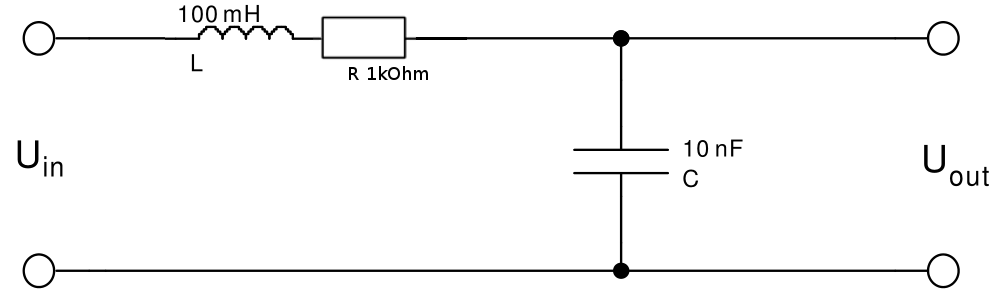
\includegraphics[scale=0.2]{4a_tiefpass_3.png}
     %\end{center}
     %\end{figure} 
     \begin{itemize}
        \item Zusätzlicher Widerstand
         \item Erwarteter Verlauf
     \end{itemize}
     \begin{equation*}
         \frac{U_{out}}{U_{in}}
         =
         \frac{Z_C}{Z_C + Z_L + R}
         =
         \frac{1}{\sqrt{\omega^4 L^2 C^2 + \omega^2 R^2 C^2 - 2 \omega^2 LC + 1}}
     \end{equation*}
\end{frame}
\begin{frame}
    \frametitle{Aufgabe 4}
    \framesubtitle{Tiefpass mit Widerstand}
     \begin{figure}[H]
     \begin{center}
             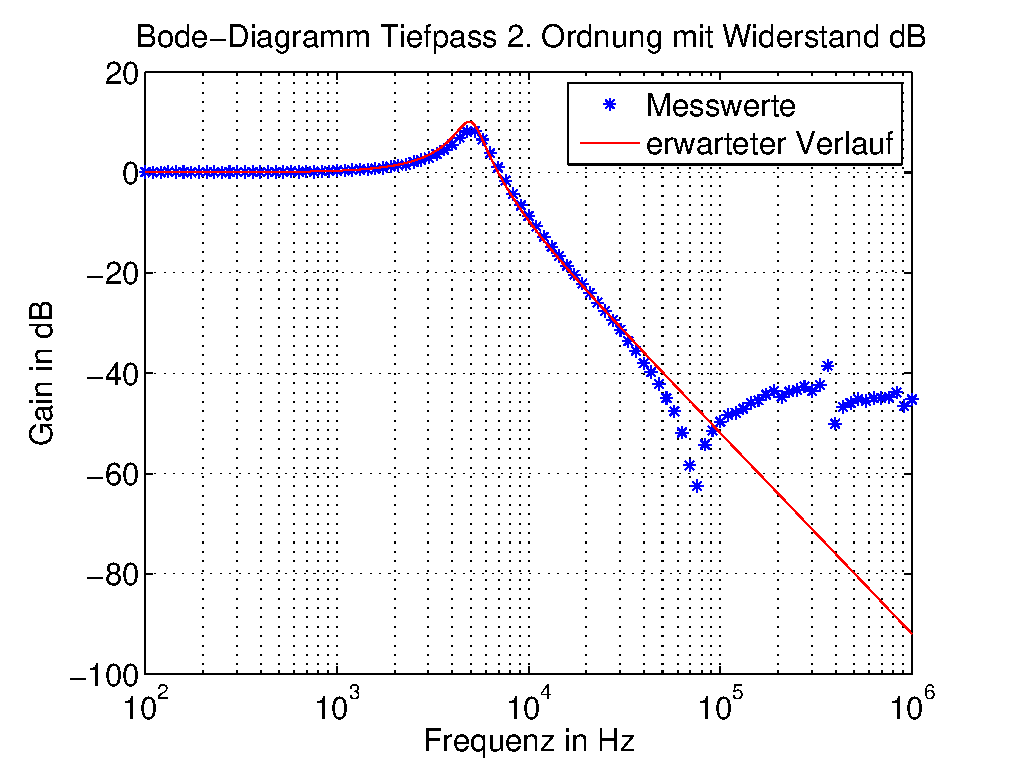
\includegraphics[scale=0.45]{./img/4a_bode_tief_dB_W.eps}
     \end{center}
     \end{figure}
     \begin{itemize}
        \item keine Asymptote
         \item Peak vor Abfall ist deutlich kleiner
         \item $R$ dämpft den Schwingkreis
     \end{itemize}
\end{frame}
\begin{frame}
    \frametitle{Aufgabe 4}
    \framesubtitle{Sperrkreisfilter}
    \begin{figure}[H]
    \begin{center}
            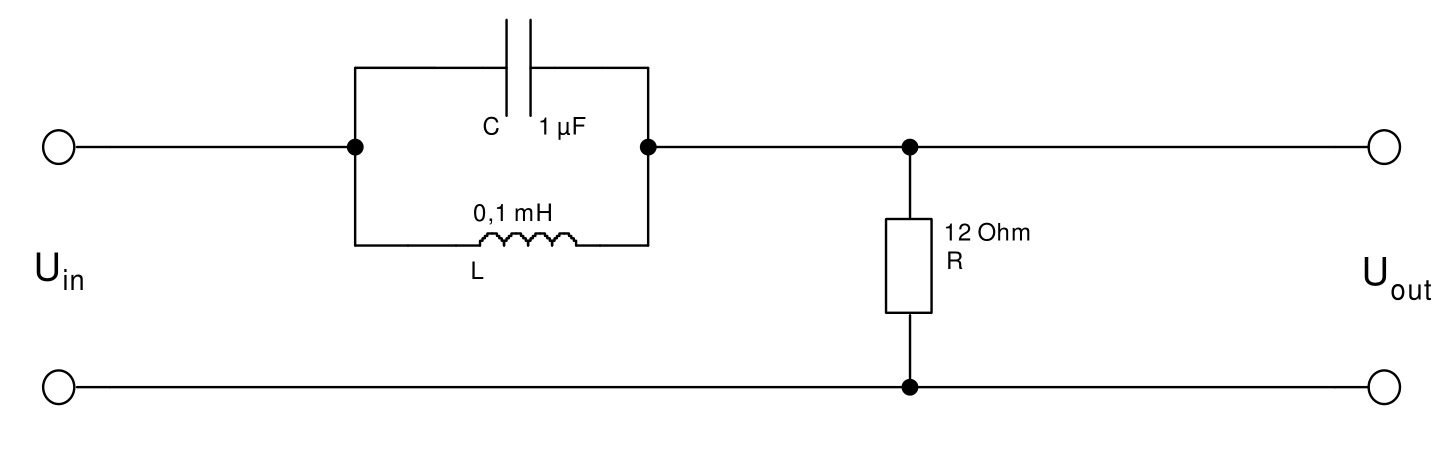
\includegraphics[scale=0.2]{./img/4b_schaltung.png}
    \end{center}
    \end{figure}
    \begin{equation*}
        \frac{U_{out}}{U_{in}}
        =
        \frac{\left\vert Z_R \right\vert}{\left\vert \frac{1}{\frac{1}{Z_C}+\frac{1}{Z_L}}
        +Z_R \right\vert }
        =
        \frac{R}{\sqrt{\left(\frac{\omega L}{\omega^2 C L +1}\right)^2 +
        R^2}}
    \end{equation*}
\end{frame}
\begin{frame}
    \frametitle{Aufgabe 4}
    \framesubtitle{Bode-Diagramm Sperrkreisfilter}
     \begin{figure}[H]
     \begin{center}
             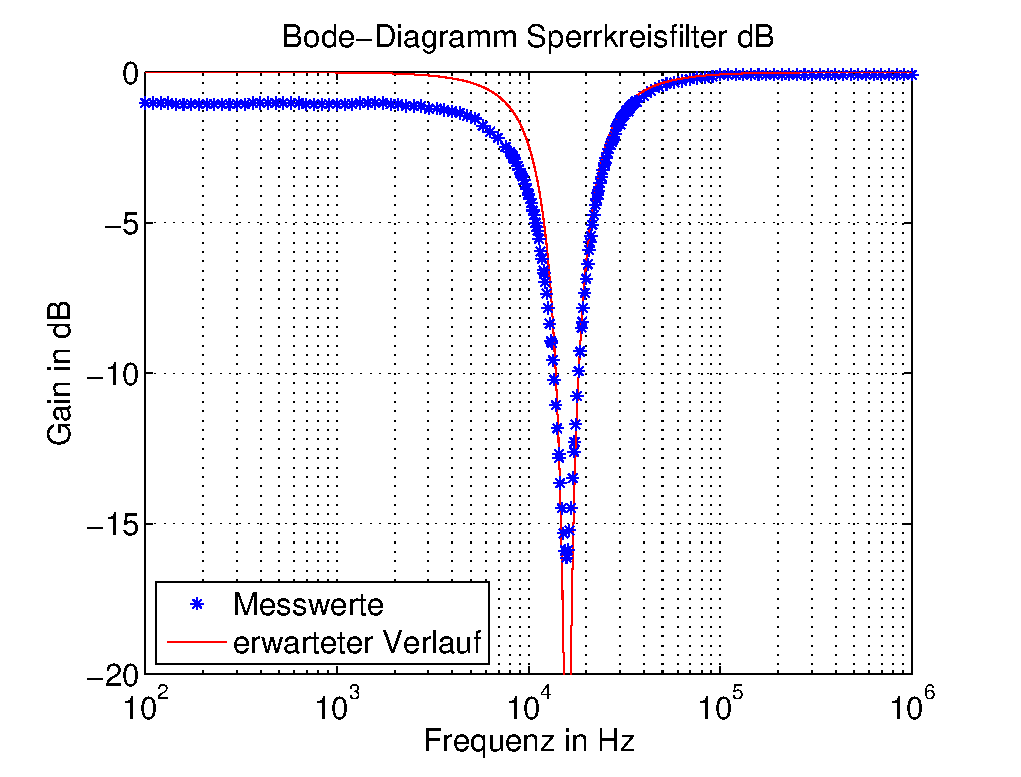
\includegraphics[scale=0.55]{./img/4b_dB.eps}
     \end{center}
     \end{figure}
\end{frame}
\begin{frame}
    \frametitle{Aufgabe 4}
    \framesubtitle{Bode-Diagramm Sperrkreisfilter}
     \begin{figure}[H]
     \begin{center}
             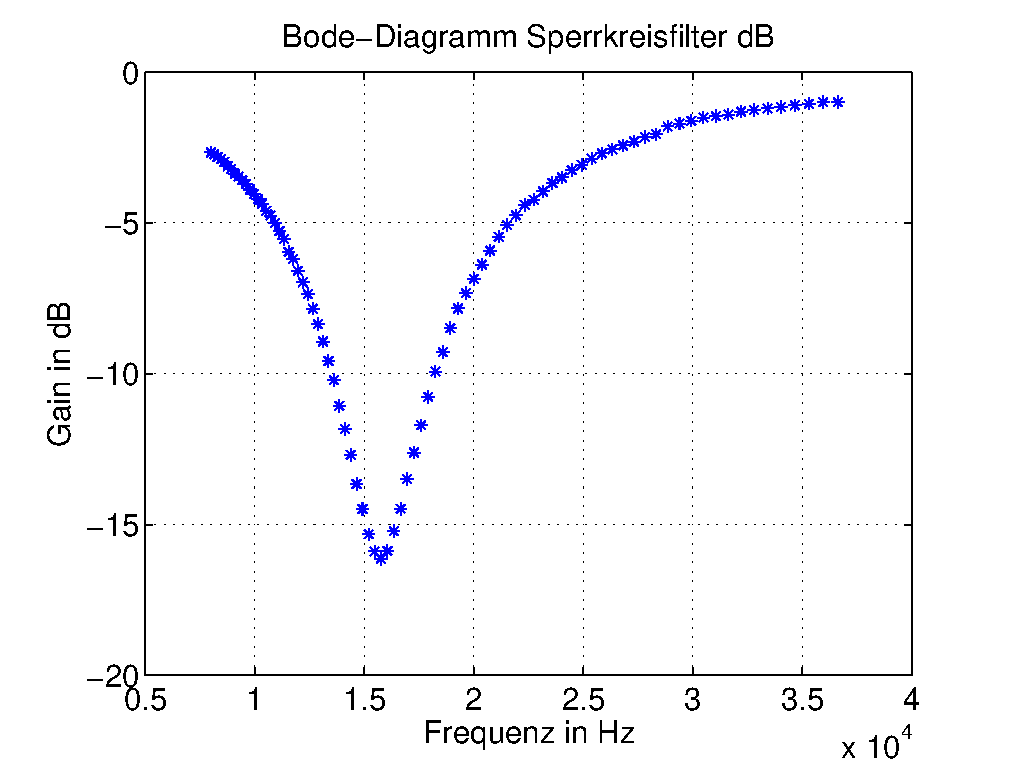
\includegraphics[scale=0.45]{./img/4b_Peak.eps}
     \end{center}
     \end{figure}
    \begin{itemize}
        \item Filtert einzelne Frequenz raus: $f \approx 16 kHz$
        \item Theorie: $f= \frac{1}{2\pi \sqrt{LC}}=15.91kHz$
    \end{itemize}
\end{frame}
\begin{frame}
    \frametitle{Aufgabe 4}
    \framesubtitle{Bode-Diagramm Sperrkreisfilter Phase}
     \begin{figure}[H]
     \begin{center}
             \includegraphics[scale=0.55]{./img/4b_Phase.eps}
     \end{center}
     \end{figure}
     \begin{itemize}
         \item Phase dreht sich beim Peak um
     \end{itemize}
\end{frame}
